\chapter[Pruebas y Resultados Experimentales]{ Pruebas y Resultados Experimentales}
\pagestyle{fancy}

Para el cumplimiento de los objetivos y verificación del correcto funcionamiento del sistema, se realizaron pruebas de funcionamiento en ambientes controlados y pruebas de campo en el Lago Ypakarai.  
\section{Prueba en ambientes controlados}
\subsection{Calibraciones de sensores}
\subsection{Muestreo en el laboratorio qu\'imica - FIUNA }
El monitorio se realiz\'o en el laboratorio de qu\'imica de la facultad de ingenier\'ia de la Universidad Nacional de Asunci\'on [QCA], sede San Lorenzo, de los par\'ametros temperatura[T], conductividad el\'ectrica[CE], potencial de hidr\'ogeno[pH].

\subsubsection{Metodolog\'ia }
Para el muestreo se tuvo en cuenta el siguiente procedimiento:  
\begin{enumerate}
    \item Se analizaron tres tipos de muestras diferentes.
    \item Cada tipo de muestra se dividen en tres recipientes.
    \item En cada recipiente se realizan un series de cinco lecturas con el sensor del laboratorio de qu\'imica y cinco lecturas con el sensor utilizado en el presente TFG.
    \item Para las lecturas se realizan un pa\'arametro a la vez, un sensor a la vez, luego de cada lectura se procede a limpiar el sensor con agua destilada y paño.
    \item Muestras:
    \begin{itemize}
        \item Muestra 1 : Agua destilada.
        \item Muestra 2 : Agua de pozo, de una red de abastecimiento de la zona.
        \item Muestra 3 : Agua de laguna de la Facultad de Ciencias Exactas y Naturales (FACEN).
    \end{itemize}
    \item Sensores laboratorio de qu\'imica
    \begin{itemize}
        \item Sensor pH 
        \begin{itemize}
            \item Marca: Ohaus
            \item Serie: ST10
            \item Intervalo de medici\'on: 0.00 – 14 [pH]
            \item Resolución de la medici\'on: 0.1   [pH]	
            \item Precisi\'on: $\pm0,1$ [pH] 
        \end{itemize}Agua destilada.
        \item Sensor CE y T
        \begin{itemize}
            \item Marca: Oaklon
            \item Serie: WD-35462-11
            \item Intervalo de medici\'on: 0.00 – 20.00 [mS/cm]
            \item Resoluci\'on: TDS 10 [ppm], 0,1 [ppt]
            \item Precisi\'on: 0,1 [pH] |0,1 [$^{\circ}$ C]
         \end{itemize}
    \end{itemize}
\end{enumerate}

\subsubsection{Muestra 1. Sensor de temperatura}
    \begin{table}[H]
        \protect\caption[Muestra 1: Destilada ]{Muestra 1: Agua de destilada.}
        \label{tab:TMuestra1}
        \centering
        \begin{tabular}{|c|c|c|}
            \hline
            \multicolumn{3}{|c|}{\textbf{Muestra 1: Agua de destilada}} \\
             \hline
            \multicolumn{3}{|c|}{\textbf{Recipiente 1}} \\
            \hline
            \textbf{Lectura}&\textbf{LSD ($^{\circ}$C)}&\textbf{Qca ($^{\circ}$C)} \\
            \hline
            {1}& $25.7$&$25.5$ \\ 
            \hline
            {2}& $25.4$&$25.5$ \\ 
            \hline
             {3}& $25.6$&$25.6$\\  
            \hline
            {4}& $25.4$&$25.5$\\ 
            \hline
            {5}& $25.2$&$25.6$ \\
            \hline
                       \multicolumn{3}{|c|}{\textbf{Recipiente 2}} \\
            \hline
            \textbf{Lectura}&\textbf{LSD ($^{\circ}$C)}&\textbf{Qca ($^{\circ}$C)} \\
            \hline
            {1}& $25.5$&$25.3$ \\ 
            \hline
            {2}& $25.4$&$25.3$ \\ 
            \hline
             {3}& $25.2$&$25.3$\\  
            \hline
            {4}& $24.8$&$25.4$\\ 
            \hline
            {5}& $24.6$&$25.4$ \\ 
            \hline
            \multicolumn{3}{|c|}{\textbf{Recipiente 3}} \\
            \hline
            \textbf{Lectura}&\textbf{LSD ($^{\circ}$C)}&\textbf{Qca´($^{\circ}$C)} \\
            \hline
            {1}& $24.6$&$25.4$ \\ 
            \hline
            {2}& $25.6$&$25.6$ \\ 
            \hline
             {3}& $25.9$&$25.6$\\  
            \hline
            {4}& $25.6$&$25.4$\\ 
            \hline
            {5}& $25.4$&$25.3$ \\ 
            \hline
        \end{tabular}
        \vspace{5mm}
        \newline
        \hfill \textbf{Fuente: }Elaboración Propia.
    \end{table}

% Grafico M1T
    \begin{figure}[H]
        \centering
        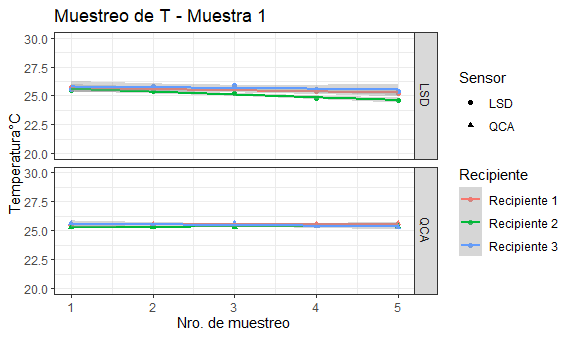
\includegraphics[width=0.75\linewidth]{Imagenes/cap4/T_M1.png}
        \caption {Muestreo de temperatura. \textbf{Fuente:}
        Elaboraci\'on Propia. }
        \label{fig:M1T}
    \end{figure}
    
\subsubsection{Muestra 1. Sensor Conductividad El\'ectrica}
    \begin{table}[H]
        \protect\caption[Muestra 1: Destilada ]{Muestra 1: Agua de destilada.}
        \label{tab:TMuestra1}
        \centering
        \begin{tabular}{|c|c|c|}
            \hline
            \multicolumn{3}{|c|}{\textbf{Muestra 1: Agua de destilada}} \\
             \hline
            \multicolumn{3}{|c|}{\textbf{Recipiente 1}} \\
            \hline
            \textbf{Lectura}&\textbf{LSD ($\mu S/cm$)}&\textbf{Qca ($\mu S/cm$)} \\
            \hline
            {1}& $0$&$0$ \\ 
            \hline
            {2}& $0$&$0$ \\ 
            \hline
             {3}& $0$&$0$\\  
            \hline
            {4}& $0$&$0$\\ 
            \hline
            {5}& $0$&$0$ \\
            \hline
                       \multicolumn{3}{|c|}{\textbf{Recipiente 2}} \\
            \hline
            \textbf{Lectura}&\textbf{LSD ($\mu S/cm$)}&\textbf{Qca ($\mu S/cm$)} \\
            \hline
            {1}& $0$&$0$ \\ 
            \hline
            {2}& $0$&$0$ \\ 
            \hline
            {3}& $0$&$0$\\  
            \hline
            {4}& $0$&$0$\\ 
            \hline
            {5}& $0$&$0$ \\
            \hline
            \multicolumn{3}{|c|}{\textbf{Recipiente 3}} \\
            \hline
            \textbf{Lectura}&\textbf{LSD ($\mu S/cm$)}&\textbf{Qca ($\mu S/cm$)} \\
            \hline
            {1}& $0$&$0$ \\ 
            \hline
            {2}& $0$&$0$ \\ 
            \hline
             {3}& $0$&$0$\\  
            \hline
            {4}& $0$&$0$\\ 
            \hline
            {5}& $0$&$0$ \\
            \hline
        \end{tabular}
        \vspace{5mm}
        \newline
        \hfill \textbf{Fuente: }Elaboración Propia.
    \end{table}

% Grafico M1CE
    \begin{figure}[H]
        \centering
        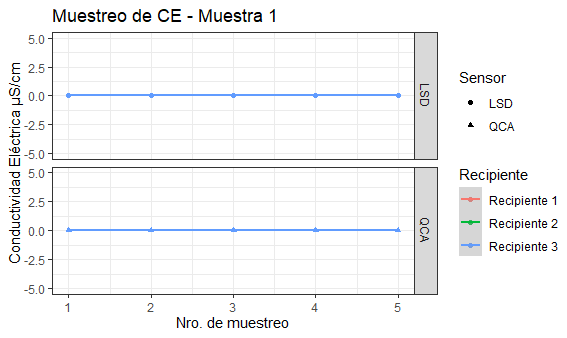
\includegraphics[width=0.75\linewidth]{Imagenes/cap4/CE_M1.png}
        \caption {Muestreo de conductividad el\'ectrica. \textbf{Fuente:}
c        Elaboraci\'on Propia. }
        \label{fig:M1CE}
    \end{figure}

\subsubsection{Muestra 1. Sensor de pH}
    \begin{table}[H]
        \protect\caption[Muestra 1: Destilada ]{Muestra 1: Agua de destilada.}
        \label{tab:TMuestra1}
        \centering
        \begin{tabular}{|c|c|c|}
            \hline
            \multicolumn{3}{|c|}{\textbf{Muestra 1: Agua de destilada}} \\
             \hline
            \multicolumn{3}{|c|}{\textbf{Recipiente 1}} \\
            \hline
            \textbf{Lectura}&\textbf{LSD ($pH$)}&\textbf{Qca ($pH$)} \\
            \hline
            {1}& $6.898$&$8.27$ \\ 
            \hline
            {2}& $6.853$&$7.86$ \\ 
            \hline
            {3}& $6.856$&$7.36$\\  
            \hline
            {4}& $6.809$&$6.82$\\ 
            \hline
            {5}& $6.715$&$6.86$ \\
            \hline
            \multicolumn{3}{|c|}{\textbf{Recipiente 2}} \\
            \hline
            \textbf{Lectura}&\textbf{LSD ($pH$)}&\textbf{Qca ($pH$)} \\
            \hline
            {1}& $6.555$&$6.59$ \\ 
            \hline
            {2}& $6.303$&$6.88$ \\ 
            \hline
            {3}& $5.919$&$6.76$\\  
            \hline
            {4}& $5.502$&$6.65$\\ 
            \hline
            {5}& $5.171$&$6.62$ \\
            \hline
            \multicolumn{3}{|c|}{\textbf{Recipiente 3}} \\
            \hline
            \textbf{Lectura}&\textbf{LSD ($pH$)}&\textbf{Qca ($pH$)} \\
            \hline
            {1}& $6.495$&$6.86$ \\ 
            \hline
            {2}& $6.440$&$6.77$ \\ 
            \hline
             {3}& $6.316$&$6.49$\\  
            \hline
            {4}& $6.711$&$6.18$\\ 
            \hline
            {5}& $6.613$&$6.37$ \\
            \hline
        \end{tabular}
        \vspace{5mm}
        \newline
        \hfill \textbf{Fuente: }Elaboración Propia.
    \end{table}

% Grafico M1Ph
    \begin{figure}[H]
        \centering
        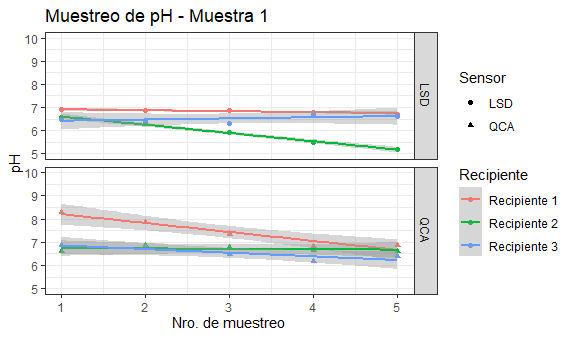
\includegraphics[width=0.75\linewidth]{Imagenes/cap4/pH_M1.png}
        \caption {Muestreo de pH. \textbf{Fuente:}
        Elaboraci\'on Propia. }
        \label{fig:M1PH}
    \end{figure}

\subsubsection{An\'alisis de Datos. Muestra 1}
% Please add the following required packages to your document preamble:

\begin{table}[H]
\protect\caption[Muestra 1: Destilada ]{Resumen de mediciones: Muestra 1.}
\label{tab:ResumenM1}
\begin{tabular}{|l|ccc|ccc|}
\hline
\multicolumn{1}{|c|}{\multirow{2}{*}{\textbf{Muestra 1}}} & \multicolumn{3}{c|}{\textbf{LSD}}                                                                                                                      & \multicolumn{3}{c|}{\textbf{QCA}}                                                                                                                       \\ \cline{2-7} 
\multicolumn{1}{|c|}{}                                    & \multicolumn{1}{c|}{\begin{tabular}[c]{@{}c@{}}T$ ^{\circ}C$\end{tabular}} & \multicolumn{1}{c|}{pH}    & \begin{tabular}[c]{@{}c@{}}CE\\ $\mu S/cm$\end{tabular} & \multicolumn{1}{c|}{\begin{tabular}[c]{@{}c@{}}T \\ $ ^{\circ}C$\end{tabular}} & \multicolumn{1}{c|}{pH}    & \begin{tabular}[c]{@{}c@{}}CE\\  $\mu S/cm$\end{tabular} \\ \hline
Mínimo                                                    & \multicolumn{1}{c|}{24.60}                                           & \multicolumn{1}{c|}{5.171} & 0                                                  & \multicolumn{1}{c|}{25.30}                                           & \multicolumn{1}{c|}{6.180} & 0                                                   \\ \hline
Máximo                                                    & \multicolumn{1}{c|}{25.90}                                           & \multicolumn{1}{c|}{6.898} & 0                                                  & \multicolumn{1}{c|}{25.60}                                           & \multicolumn{1}{c|}{8.27}  & 0                                                   \\ \hline
Promedio                                                  & \multicolumn{1}{c|}{25.41}                                           & \multicolumn{1}{c|}{6.410} & 0                                                  & \multicolumn{1}{c|}{25.45}                                           & \multicolumn{1}{c|}{6.889} & 0                                                   \\ \hline
\end{tabular}
\end{table}


\begin{table}[H]
\protect\caption[Muestra 1: Destilada ]{Estad\'issticas de mediciones: Muestra 1.}
\label{tab:TAnalisisM1}
\begin{tabular}{|l|ccc|ccc}
\hline
\textbf{Muestra 1  }& \multicolumn{3}{c|}{LSD}                                                                                                                                   & \multicolumn{3}{c|}{QCA}                                                                                                                                                        \\ \hline
\begin{tabular}[c]{@{}l@{}}Análisis de datos \\ obtenidos\end{tabular} & \multicolumn{1}{c|}{\begin{tabular}[c]{@{}c@{}}T \\$ ^{\circ}C$\end{tabular}} & \multicolumn{1}{c|}{pH}        & \begin{tabular}[c]{@{}c@{}}CE\\ $\mu S/cm$\end{tabular} & \multicolumn{1}{c|}{\begin{tabular}[c]{@{}c@{}}T \\$ ^{\circ}C$\end{tabular}} & \multicolumn{1}{c|}{pH}        & \multicolumn{1}{c|}{\begin{tabular}[c]{@{}c@{}}CE\\ $\mu S/cm$\end{tabular}} \\ \hline
Desviación Est\'andar                                                             & \multicolumn{1}{c|}{0.349}                                       & \multicolumn{1}{c|}{0.511} & 0                                                  & \multicolumn{1}{c|}{0.118}                                       & \multicolumn{1}{c|}{0.551} & \multicolumn{1}{c|}{0}                                                  \\ \hline
Varianza                                                                        & \multicolumn{1}{c|}{0.122}                                       & \multicolumn{1}{c|}{0.261} & 0                                                  & \multicolumn{1}{c|}{0.014}                                      & \multicolumn{1}{c|}{0.304} & \multicolumn{1}{c|}{0}                                                  \\ \hline
\begin{tabular}[c]{@{}l@{}}Coeficiente de \\ Variación\end{tabular}             & \multicolumn{1}{c|}{1.375}                                        & \multicolumn{1}{c|}{7.984}  & 0                                                  & \multicolumn{1}{c|}{0.466}                                       & \multicolumn{1}{c|}{8.006}  & \multicolumn{1}{c|}{0}                                                  \\ \hline
Error Estándar                                                                  & \multicolumn{1}{c|}{0.090}                                      & \multicolumn{1}{c|}{0.132} & 0                                                  & \multicolumn{1}{c|}{0.0306}                                      & \multicolumn{1}{c|}{0.142} & \multicolumn{1}{c|}{0}                                                  \\ \hline
Covarianza                                                                      & \multicolumn{1}{c|}{0.0125}                                      & \multicolumn{1}{c|}{0.111} & 0                                                  &                                                                      &                                &                                                                         \\ \cline{1-4}
Correlación                                                                     & \multicolumn{1}{c|}{0.301}                                       & \multicolumn{1}{c|}{0.395} & 0                                                  &                                                                      &                                &                                                                         \\ \cline{1-4}
\end{tabular}
\vspace{5mm}
\newline
\hfill \textbf{Fuente: }Elaboración Propia.
\end{table}


%% Muestra nro 2: Agua de Pozo

\subsubsection{Muestra 2.Temperatura}
    \begin{table}[H]
        \protect\caption[Muestra 2: Agua de pozo ]{Muestra 2: Agua de pozo.}
        \label{tab:TMuestra2}
        \centering
        \begin{tabular}{|c|c|c|}
            \hline
            \multicolumn{3}{|c|}{\textbf{Muestra 2: Agua de pozo.}} \\
             \hline
            \multicolumn{3}{|c|}{\textbf{Recipiente 1}} \\
            \hline
            \textbf{Lectura}&\textbf{LSD($^{\circ}$C)}&\textbf{Qca($^{\circ}$C)} \\
            \hline
            {1}& $23.6$&$25.1$ \\ 
            \hline
            {2}& $22.9$&$24.9$ \\ 
            \hline
             {3}& $22.6$&$24.8$\\  
            \hline
            {4}& $22.5$&$24.6$\\ 
            \hline
            {5}& $22.3$&$24.6$ \\
            \hline
                       \multicolumn{3}{|c|}{\textbf{Recipiente 2}} \\
            \hline
            \textbf{Lectura}&\textbf{LSD($^{\circ}$C)}&\textbf{Qca($^{\circ}$C)} \\
            \hline
            {1}& $24.4$&$24.4$ \\ 
            \hline
            {2}& $24.0$&$24.2$ \\ 
            \hline
             {3}& $23.9$&$24.0$\\  
            \hline
            {4}& $23.9$&$23.9$\\ 
            \hline
            {5}& $23.8$&$23.9$ \\ 
            \hline
            \multicolumn{3}{|c|}{\textbf{Recipiente 3}} \\
            \hline
            \textbf{Lectura}&\textbf{LSD($^{\circ}$C)}&\textbf{Qca($^{\circ}$C)} \\
            \hline
            {1}& $22.2$&$23.9$ \\ 
            \hline
            {2}& $21.9$&$24.0$ \\ 
            \hline
             {3}& $21.5$&$23.8$\\  
            \hline
            {4}& $21.4$&$23.7$\\ 
            \hline
            {5}& $21.2$&$23.6$ \\ 
            \hline
        \end{tabular}
        \vspace{5mm}
        \newline
        \hfill \textbf{Fuente: }Elaboración Propia.
    \end{table}

% Gráfico M2T
    \begin{figure}[H]
        \centering
        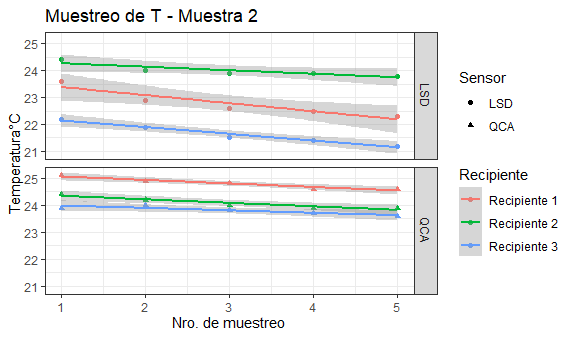
\includegraphics[width=0.75\linewidth]{Imagenes/cap4/T_M2.png}
        \caption {Muestreo de temperatura. \textbf{Fuente:}
        Elaboraci\'on Propia. }
        \label{fig:M2T}
    \end{figure}

\subsubsection{Muestra 2. Sensor Conductividad El\'ectrica }
    \begin{table}[H]
        \protect\caption[Muestra 2: Agua de pozo ]{Muestra 2: Agua de pozo.}
        \label{tab:CEMuestra2}
        \centering
        \begin{tabular}{|c|c|c|}
            \hline
            \multicolumn{3}{|c|}{\textbf{Muestra 2: Agua de pozo}} \\
             \hline
            \multicolumn{3}{|c|}{\textbf{Recipiente 1}} \\
            \hline
            \textbf{Lectura}&\textbf{LSD ($\mu S/cm$)}&\textbf{Qca ($\mu S/cm$)} \\
            \hline
            {1}& $81.39$&$100$ \\ 
            \hline
            {2}& $80.12$&$90$ \\ 
            \hline
             {3}&$80.05$&$90$\\  
            \hline
            {4}& $80.55$&$100$\\ 
            \hline
            {5}& $80.10$&$90$ \\
            \hline
                       \multicolumn{3}{|c|}{\textbf{Recipiente 2}} \\
            \hline
            \textbf{Lectura}&\textbf{LSD ($\mu S/cm$)}&\textbf{Qca ($\mu S/cm$)} \\
            \hline
            {1}& $80.32$&$80$ \\ 
            \hline
            {2}& $80.36$&$80$ \\ 
            \hline
             {3}&$80.40$&$80$\\  
            \hline
            {4}& $80.45$&$80$\\ 
            \hline
            {5}& $80.49$&$80$ \\ 
            \hline
            \multicolumn{3}{|c|}{\textbf{Recipiente 3}} \\
            \hline
            \textbf{Lectura}&\textbf{LSD ($\mu S/cm$)}&\textbf{Qca($\mu S/cm$)} \\
            \hline
            {1}& $119.60$&$130$ \\ 
            \hline
            {2}& $110.30$&$130$ \\ 
            \hline
             {3}&$118.90$&$130$\\  
            \hline
            {4}& $117.10$&$130$\\ 
            \hline
            {5}& $118.40$&$130$ \\ 
            \hline
        \end{tabular}
        \vspace{5mm}
        \newline
        \hfill \textbf{Fuente: }Elaboración Propia.
    \end{table}

% Gráfico M2CE
    \begin{figure}[H]
        \centering
        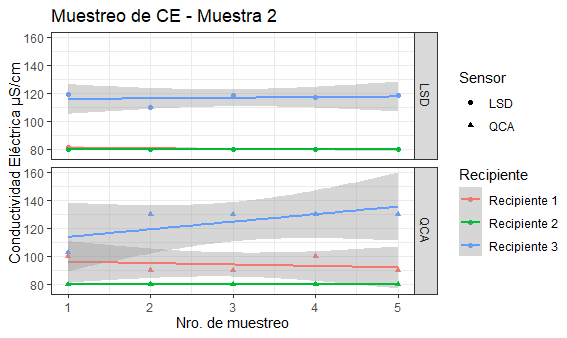
\includegraphics[width=0.75\linewidth]{Imagenes/cap4/CE_M2.png}
        \caption {Muestreo de conductividad el\'ectrica. \textbf{Fuente:}
        Elaboraci\'on Propia. }
        \label{fig:M2CE}
    \end{figure}

\subsubsection{Muestra 2. Sensor de pH}
    \begin{table}[H]
        \protect\caption[Muestra 2: Agua de pozo ]{Muestra 2: Agua de pozo.}
        \label{tab:phMuestra2}
        \centering
        \begin{tabular}{|c|c|c|}
            \hline
            \multicolumn{3}{|c|}{\textbf{Muestra 2: Agua de pozo.}} \\
             \hline
            \multicolumn{3}{|c|}{\textbf{Recipiente 1}} \\
            \hline
            \textbf{Lectura}&\textbf{LSD ($pH$)}&\textbf{Qca ($pH$)} \\
            \hline
            {1}& $5.569$&$6.12$ \\ 
            \hline
            {2}& $5.513$&$6.15$ \\ 
            \hline
            {3}& $5.458$&$6.13$\\  
            \hline
            {4}& $5.402$&$6.17$\\ 
            \hline
            {5}& $5.498$&$6.20$ \\
            \hline
            \multicolumn{3}{|c|}{\textbf{Recipiente 2}} \\
            \hline
            \textbf{Lectura}&\textbf{LSD ($pH$)}&\textbf{Qca ($pH$)} \\
            \hline
            {1}& $5.157$&$5.94$ \\ 
            \hline
            {2}& $5.251$&$5.96$ \\ 
            \hline
            {3}& $5.552$&$5.98$\\  
            \hline
            {4}& $5.595$&$6.03$\\ 
            \hline
            {5}& $5.551$&$6.01$ \\
            \hline
            \multicolumn{3}{|c|}{\textbf{Recipiente 3}} \\
            \hline
            \textbf{Lectura}&\textbf{LSD ($pH$)}&\textbf{Qca ($pH$)} \\
            \hline
            {1}& $5.582$&$5.91$ \\ 
            \hline
            {2}& $5.624$&$6.04$ \\ 
            \hline
             {3}&$5.732$&$6.11$\\  
            \hline
            {4}& $5.918$&$6.09$\\ 
            \hline
            {5}& $5.936$&$6.18$ \\
            \hline
        \end{tabular}
        \vspace{5mm}
        \newline
        \hfill \textbf{Fuente: }Elaboración Propia.
    \end{table}

% Gráfico M2pH
    \begin{figure}[H]
        \centering
        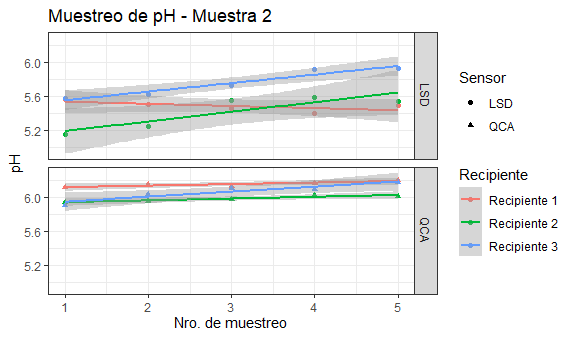
\includegraphics[width=0.75\linewidth]{Imagenes/cap4/pH_M2.png}
        \caption {Muestreo de pH. \textbf{Fuente:}
        Elaboraci\'on Propia. }
        \label{fig:M2PH}
    \end{figure}

\subsection{An\'alsis de Datos. Muestra 2}

% Please add the following required packages to your document preamble:
% \usepackage{multirow}
\begin{table}[H]
\begin{tabular}{|l|ccc|ccc|}
\hline
\multicolumn{1}{|c|}{\multirow{2}{*}{\textbf{Muestra 2}}} & \multicolumn{3}{c|}{\textbf{LSD}}                                                                                                                      & \multicolumn{3}{c|}{\textbf{QCA}}                                                                                                                       \\ \cline{2-7} 
\multicolumn{1}{|c|}{}                                    & \multicolumn{1}{c|}{\begin{tabular}[c]{@{}c@{}}T \\ $^{\circ} C$\end{tabular}} & \multicolumn{1}{c|}{$pH$}    & \begin{tabular}[c]{@{}c@{}}CE\\ $\mu S/cm$\end{tabular} & \multicolumn{1}{c|}{\begin{tabular}[c]{@{}c@{}}T \\ $^{\circ} C$\end{tabular}} & \multicolumn{1}{c|}{$pH$}    & \begin{tabular}[c]{@{}c@{}}CE\\  $\mu S/cm$\end{tabular} \\ \hline
Mínimo                                                    & \multicolumn{1}{c|}{21.20}                                           & \multicolumn{1}{c|}{5.157} & 80.05                                              & \multicolumn{1}{c|}{23.60}                                           & \multicolumn{1}{c|}{5.910} & 80.0                                                \\ \hline
Máximo                                                    & \multicolumn{1}{c|}{24.40}                                           & \multicolumn{1}{c|}{5.936} & 119.60                                             & \multicolumn{1}{c|}{25.10}                                           & \multicolumn{1}{c|}{6.200} & 130.0                                               \\ \hline
Promedio                                                  & \multicolumn{1}{c|}{22.81}                                           & \multicolumn{1}{c|}{5.556} & 92.57                                              & \multicolumn{1}{c|}{24.23}                                           & \multicolumn{1}{c|}{6.068} & 101.3                                               \\ \hline
\end{tabular}
\end{table}

\begin{table}[H]
\protect\caption[Muestra 2: Agua de pozo ]{Resumen de mediciones: Muestra 2.}
\begin{tabular}{|l|ccc|ccc}
\hline
Muestra 2                                                                       & \multicolumn{3}{c|}{LSD}                                                                                                                                   & \multicolumn{3}{c|}{QCA}                                                                                                                                                        \\ \hline
\textbf{\begin{tabular}[c]{@{}l@{}}Análisis de datos \\ obtenidos\end{tabular}} & \multicolumn{1}{c|}{\begin{tabular}[c]{@{}c@{}}T \\ $^{\circ} C$\end{tabular}} & \multicolumn{1}{c|}{pH}        & \begin{tabular}[c]{@{}c@{}}CE\\ $\mu S/cm$\end{tabular} & \multicolumn{1}{c|}{\begin{tabular}[c]{@{}c@{}}T \\ $^{\circ} C$\end{tabular}} & \multicolumn{1}{c|}{pH}        & \multicolumn{1}{c|}{\begin{tabular}[c]{@{}c@{}}CE\\ $\mu S/cm$\end{tabular}} \\ \hline
Desviación Est\'andar                                                             & \multicolumn{1}{c|}{0.349}                                       & \multicolumn{1}{c|}{0.511} & 0                                                  & \multicolumn{1}{c|}{0.118}                                       & \multicolumn{1}{c|}{0.551} & \multicolumn{1}{c|}{0}                                                  \\ \hline
Varianza                                                                        & \multicolumn{1}{c|}{0.122}                                       & \multicolumn{1}{c|}{0.262} & 0                                                  & \multicolumn{1}{c|}{0.014}                                      & \multicolumn{1}{c|}{0.304} & \multicolumn{1}{c|}{0}                                                  \\ \hline
\begin{tabular}[c]{@{}l@{}}Coeficiente de \\ Variación\end{tabular}             & \multicolumn{1}{c|}{1.375}                                        & \multicolumn{1}{c|}{7.984}  & 0                                                  & \multicolumn{1}{c|}{0.466}                                       & \multicolumn{1}{c|}{8.006}  & \multicolumn{1}{c|}{0}                                                  \\ \hline
Error Estándar                                                                  & \multicolumn{1}{c|}{0.090}                                      & \multicolumn{1}{c|}{0.132} & 0                                                  & \multicolumn{1}{c|}{0.0306}                                      & \multicolumn{1}{c|}{0.142} & \multicolumn{1}{c|}{0}                                                  \\ \hline
Covarianza                                                                      & \multicolumn{1}{c|}{0.0125}                                      & \multicolumn{1}{c|}{0.1115} & 0                                                  &                                                                      &                                &                                                                         \\ \cline{1-4}
Correlación                                                                     & \multicolumn{1}{c|}{0.302}                                       & \multicolumn{1}{c|}{0.395} & 0                                                  &                                                                      &                                &                                                                         \\ \cline{1-4}
\end{tabular}
\end{table}

\subsubsection{Muestra 3. Sensor de Temperatura}
  \begin{table}[H]
        \protect\caption[Muestra 3: Agua de laguna]{Muestra 3: Agua de laguna.}
        \label{tab:TMuestra3}
        \centering
        \begin{tabular}{|c|c|c|}
            \hline
            \multicolumn{3}{|c|}{\textbf{Muestra 3: Agua de laguna.}} \\
             \hline
            \multicolumn{3}{|c|}{\textbf{Recipiente 1}} \\
            \hline
            \textbf{Lectura}&\textbf{LSD ($^{\circ} C$)}&\textbf{Qca ($^{\circ} C$)} \\
            \hline
            {1}& $22.3$&$22.1$ \\ 
            \hline
            {2}& $22.2$&$22.3$ \\ 
            \hline
            {3}& $22.3$&$22.1$\\  
            \hline
            {4}& $22.1$&$21.9$\\ 
            \hline
            {5}& $22.1$&$21.8$ \\
            \hline
            \multicolumn{3}{|c|}{\textbf{Recipiente 2}} \\
            \hline
            \textbf{Lectura}&\textbf{LSD ($^{\circ} C$)}&\textbf{Qca ($^{\circ} C$)} \\
            \hline
            {1}& $22.7$&$21.8$ \\ 
            \hline
            {2}& $22.7$&$22.9$ \\ 
            \hline
            {3}& $22.7$&$22.9$\\  
            \hline
            {4}& $22.7$&$22.7$\\ 
            \hline
            {5}& $22.7$&$22.7$ \\
            \hline
            \multicolumn{3}{|c|}{\textbf{Recipiente 3}} \\
            \hline
            \textbf{Lectura}&\textbf{LSD ($^{\circ} C$)}&\textbf{Qca ($^{\circ} C$)} \\
            \hline
            {1}& $22.7$&$22.2$ \\ 
            \hline
            {2}& $22.8$&$22.2$ \\ 
            \hline
             {3}&$22.8$&$22.2$\\  
            \hline
            {4}& $22.9$&$22.3$\\ 
            \hline
            {5}& $22.9$&$22.4$ \\
            \hline
        \end{tabular}
        \vspace{5mm}
        \newline
        \hfill \textbf{Fuente: }Elaboración Propia.
    \end{table}

% Gráfico M3T
    \begin{figure}[H]
        \centering
        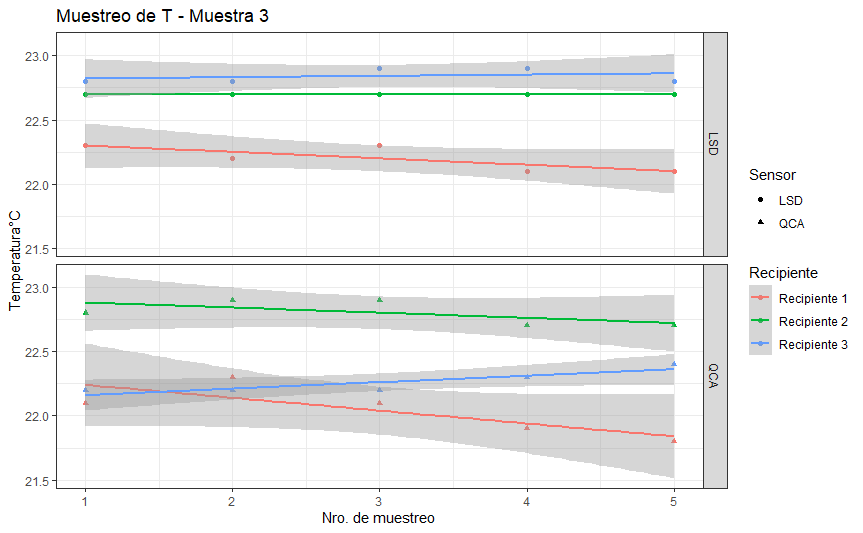
\includegraphics[width=0.75\linewidth]{Imagenes/cap4/T_M3.png}
        \caption {Muestreo de pH. \textbf{Fuente:}
        Elaboraci\'on Propia. }
        \label{fig:M3T}
    \end{figure}

\subsubsection{Muestra 3. Sensor Conductividad El\'ectrica}

  \begin{table}[H]
        \protect\caption[Muestra 3: Agua de laguna]{Muestra 3: Agua de laguna.}
        \label{tab:CEMuestra3}
        \centering
        \begin{tabular}{|c|c|c|}
            \hline
            \multicolumn{3}{|c|}{\textbf{Muestra 3: Agua de laguna.}} \\
             \hline
            \multicolumn{3}{|c|}{\textbf{Recipiente 1}} \\
            \hline
            \textbf{Lectura}&\textbf{LSD ($\mu S/cm$)}&\textbf{Qca ($\mu S/cm$)} \\
            \hline
            {1}& $36.35$&$50$ \\ 
            \hline
            {2}& $35.18$&$52$ \\ 
            \hline
            {3}& $35.15$&$50$\\  
            \hline
            {4}& $34.87$&$50$\\ 
            \hline
            {5}& $33.70$&$51$ \\
            \hline
            \multicolumn{3}{|c|}{\textbf{Recipiente 2}} \\
            \hline
            \textbf{Lectura}&\textbf{LSD ($\mu S/cm$)}&\textbf{Qca ($\mu S/cm$)} \\
            \hline
            {1}& $32.24$&$52$ \\ 
            \hline
            {2}& $34.01$&$51$ \\ 
            \hline
            {3}& $34.13$&$50$\\  
            \hline
            {4}& $33.03$&$53$\\ 
            \hline
            {5}& $32.75$&$52$ \\
            \hline
            \multicolumn{3}{|c|}{\textbf{Recipiente 3}} \\
            \hline
            \textbf{Lectura}&\textbf{LSD ($\mu S/cm$)}&\textbf{Qca ($\mu S/cm$)} \\
            \hline
            {1}& $37.39$&$51$ \\ 
            \hline
            {2}& $36.75$&$50$ \\ 
            \hline
             {3}&$39.31$&$50$\\  
            \hline
            {4}& $44.40$&$53$\\ 
            \hline
            {5}& $42.57$&$52$ \\
            \hline
        \end{tabular}
        \vspace{5mm}
        \newline
        \hfill \textbf{Fuente: }Elaboración Propia.
    \end{table}

% Gráfico CE3T
    \begin{figure}[H]
        \centering
        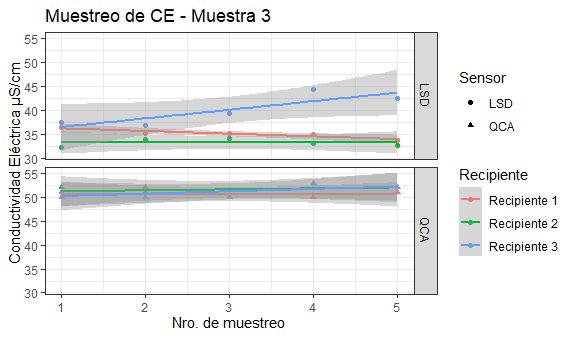
\includegraphics[width=0.75\linewidth]{Imagenes/cap4/CE_M3.png}
        \caption {Muestreo de conductividad el\'ectrica. \textbf{Fuente:}
        Elaboraci\'on Propia. }
        \label{fig:M3CE}
    \end{figure}

\subsubsection{Muestra 3. Sensor de pH}
%%%%% noooo
  \begin{table}[H]
        \protect\caption[Muestra 3: Agua de laguna]{Muestra 3: Agua de laguna.}
        \label{tab:TMuestra3}
        \centering
        \begin{tabular}{|c|c|c|}
            \hline
            \multicolumn{3}{|c|}{\textbf{Muestra 3: Agua de laguna.}} \\
             \hline
            \multicolumn{3}{|c|}{\textbf{Recipiente 1}} \\
            \hline
            \textbf{Lectura}&\textbf{LSD ($pH$)}&\textbf{Qca ($pH$)} \\
            \hline
            {1}& $6.302$&$6.99$ \\ 
            \hline
            {2}& $6.285$&$6.98$ \\ 
            \hline
            {3}& $6.318$&$6.96$\\  
            \hline
            {4}& $6.253$&$7.00$\\ 
            \hline
            {5}& $6.081$&$6.93$ \\
            \hline
            \multicolumn{3}{|c|}{\textbf{Recipiente 2}} \\
            \hline
            \textbf{Lectura}&\textbf{LSD ($pH$)}&\textbf{Qca ($pH$)} \\
            \hline
            {1}& $6.255$&$7.19$ \\ 
            \hline
            {2}& $6.265$&$7.14$ \\ 
            \hline
            {3}& $6.265$&$7.13$\\  
            \hline
            {4}& $6.138$&$7.10$\\ 
            \hline
            {5}& $6.138$&$7.20$ \\
            \hline
            \multicolumn{3}{|c|}{\textbf{Recipiente 3}} \\
            \hline
            \textbf{Lectura}&\textbf{LSD ($pH$)}&\textbf{Qca ($pH$)} \\
            \hline
            {1}& $6.482$&$6.61$ \\ 
            \hline
            {2}& $6.488$&$6.74$ \\ 
            \hline
             {3}&$6.532$&$7.07$\\  
            \hline
            {4}& $6.538$&$7.01$\\ 
            \hline
            {5}& $6.522$&$7.20$ \\
            \hline
        \end{tabular}
        \vspace{5mm}
        \newline
        \hfill \textbf{Fuente: }Elaboración Propia.
    \end{table}

% Gráfico M3PH
\begin{figure}[H]
        \centering
        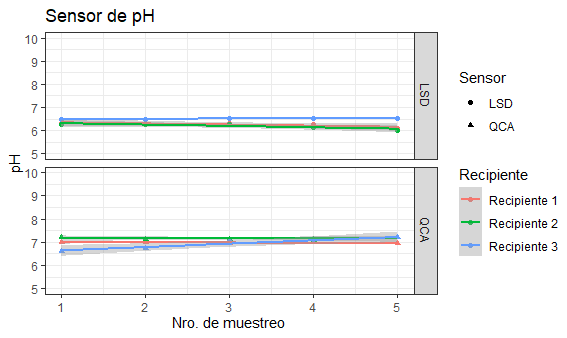
\includegraphics[width=0.75\linewidth]{Imagenes/cap4/pH_M3.png}
        \caption {Muestreo de pH. \textbf{Fuente:}
        Elaboraci\'on Propia. }
        \label{fig:M3PH}
    \end{figure}

\subsection{An\'alsis de Datos. Muestra 3}

% Please add the following required packages to your document preamble:
% \usepackage{multirow}
\begin{table}[H]
\begin{tabular}{|l|ccc|ccc|}
\hline
\multicolumn{1}{|c|}{\multirow{2}{*}{\textbf{Muestra 3}}} & \multicolumn{3}{c|}{\textbf{LSD}}                                                                                                                      & \multicolumn{3}{c|}{\textbf{QCA}}                                                                                                                       \\ \cline{2-7} 
\multicolumn{1}{|c|}{}                                    & \multicolumn{1}{c|}{\begin{tabular}[c]{@{}c@{}}T \\ $^{\circ} C$\end{tabular}} & \multicolumn{1}{c|}{$pH$}    & \begin{tabular}[c]{@{}c@{}}CE\\ $\mu S/cm$\end{tabular} & \multicolumn{1}{c|}{\begin{tabular}[c]{@{}c@{}}T \\ $^{\circ} C$\end{tabular}} & \multicolumn{1}{c|}{$pH$}    & \begin{tabular}[c]{@{}c@{}}CE\\  $\mu S/cm$\end{tabular} \\ \hline
Mínimo                                                    & \multicolumn{1}{c|}{22.10}                                           & \multicolumn{1}{c|}{6.023} & 32.24                                              & \multicolumn{1}{c|}{21.80}                                           & \multicolumn{1}{c|}{6.610} & 50.00                                               \\ \hline
Máximo                                                    & \multicolumn{1}{c|}{22.90}                                           & \multicolumn{1}{c|}{6.538} & 44.40                                              & \multicolumn{1}{c|}{22.90}                                           & \multicolumn{1}{c|}{7.20}  & 53.00                                               \\ \hline
Promedio                                                  & \multicolumn{1}{c|}{22.58}                                           & \multicolumn{1}{c|}{6.316} & 36.12                                              & \multicolumn{1}{c|}{22.37}                                           & \multicolumn{1}{c|}{7.017} & 51.13                                               \\ \hline
\end{tabular}
\end{table}

\begin{table}[H]
\begin{tabular}{|l|ccc|ccc}
\hline
Muestra 3                                                                       & \multicolumn{3}{c|}{LSD}                                                                                                                                 & \multicolumn{3}{c|}{QCA}                                                                                                                                                     \\ \hline
\textbf{\begin{tabular}[c]{@{}l@{}}Análisis de datos \\ obtenidos\end{tabular}} & \multicolumn{1}{c|}{\begin{tabular}[c]{@{}c@{}}T \\ $^{\circ} C$\end{tabular}} & \multicolumn{1}{c|}{pH}        & \begin{tabular}[c]{@{}c@{}}CE\\ $\mu S/cm$\end{tabular} & \multicolumn{1}{c|}{\begin{tabular}[c]{@{}c@{}}T \\ $^{\circ} C$\end{tabular}} & \multicolumn{1}{c|}{pH}        & \multicolumn{1}{c|}{\begin{tabular}[c]{@{}c@{}}CE\\ $\mu S/cm$\end{tabular}} \\ \hline
Desviación Estandar                                                             & \multicolumn{1}{c|}{0.291}                                           & \multicolumn{1}{c|}{0.165}   & 3.545                                              & \multicolumn{1}{c|}{0.354}                                           & \multicolumn{1}{c|}{0.167}  & \multicolumn{1}{c|}{1.125}                                              \\ \hline
Varianza                                                                        & \multicolumn{1}{c|}{0.0845}                                          & \multicolumn{1}{c|}{0.027}   & 12.57                                              & \multicolumn{1}{c|}{0.125}                                           & \multicolumn{1}{c|}{0.0279} & \multicolumn{1}{c|}{1.267}                                              \\ \hline
\begin{tabular}[c]{@{}l@{}}Coeficiente de \\ Variación\end{tabular}             & \multicolumn{1}{c|}{1.287}                                           & \multicolumn{1}{c|}{2.616}   & 9.816                                              & \multicolumn{1}{c|}{1.582}                                           & \multicolumn{1}{c|}{2.379}  & \multicolumn{1}{c|}{2.201}                                              \\ \hline
Error Estándar                                                                  & \multicolumn{1}{c|}{0.075}                                           & \multicolumn{1}{c|}{0.0426}  & 0.915                                              & \multicolumn{1}{c|}{0.0914}                                          & \multicolumn{1}{c|}{0.043}  & \multicolumn{1}{c|}{0.290}                                              \\ \hline
Covarianza                                                                      & \multicolumn{1}{c|}{0.0564}                                          & \multicolumn{1}{c|}{-0.351}  & 0.157                                              &                                                                      &                             &                                                                         \\ \cline{1-4}
Correlación                                                                     & \multicolumn{1}{c|}{0.5483}                                          & \multicolumn{1}{c|}{-0.0096} & 0.628                                              &                                                                      &                             &                                                                         \\ \cline{1-4}
\end{tabular}
\end{table}



% resumen de mediciones

%Estadistica de mediciones

\section{Pruebas de campo}
\section{Interfaz de monitoreo}
